\chapter{Sequences in Calculus}

We have introduced sequences in a previous chapter. Now, we will 
examine them in more detail in a calculus context. You already know 
about arithmetic and geometric sequences, but not all sequences can 
be classified as arithmetic or geometric. Take the famous Fibonacci 
sequence, \{1, 1, 2, 3, 5, 8, ...\}, which can be explicitly defined 
as $a_n = a_{n-1} + a_{n-2}$, with $a_1 = a_2 = 1$. There is no 
common difference or common ratio, so the Fibonacci sequence is not 
arithmetic or geometric. Another example is $a_n = 
\sin{\frac{n\pi}{6}}$, which will cycle through a set of values. 

Sequences have many real-world applications, including compound 
interest and modeling population growth. In later chapters, you will 
learn that the sum of all the values in a sequence is a series and 
how to use series to describe functions. In order to be able to do 
all that, first we need to talk in-depth about sequences. 

Some sequences are defined explicitly, like $a_n = 
\sin{\frac{n\pi}{6}}$, while others are defined recursively, like $a_n 
= a_{n-1} + a_{n-2}$. 

Example: Write the first 5 terms for the explicitly defined sequence 
$a_n = \frac{n}{n+1}$.

Solution: We can construct a table to keep track of our work:
\begin{center}
\begin{tabular}{|c|c|c|}\hline
$n$ & work & $a_n$\\
\hline
1 & $\frac{1}{1+1}$ & $\frac{1}{2}$\\
\hline
2 & $\frac{2}{2+1}$ & $\frac{2}{3}$\\
\hline
3 & $\frac{3}{3+1}$ & $\frac{3}{4}$\\
\hline
4 & $\frac{4}{4+1}$ & $\frac{4}{5}$\\
\hline
5 & $\frac{5}{5+1}$ & $\frac{5}{6}$\\
\hline
\end{tabular}
\end{center}

So the first five terms are \{$\frac{1}{2}$, $\frac{2}{3}$, 
$\frac{3}{4}$, $\frac{4}{5}$, $\frac{5}{6}$\}. 

\begin{Exercise}[label = seqcalc1]
Write the first 5 terms for each sequence. 
\begin{enumerate}
\item $a_n = \frac{2^n}{2n+1}$
\item $a_n = \cos{\frac{n\pi}{2}}$
\item $a_1 = 1$, $a_{n+1} = 5a_n-3$
\item $a_1 = 6$, $a_{n+1} = \frac{a_n}{n+1}$
\end{enumerate}
\end{Exercise}

\begin{Answer}[ref=seqcalc1]
\begin{enumerate}
\item $\frac{2}{3}$, $\frac{4}{5}$, $\frac{8}{7}$, $\frac{16}{9}$, 
$\frac{32}{11}$
\item 0, -1, 0, 1, 0
\item 1, 2, 7, 32, 157
\item 6, 3, 1, $\frac{1}{4}$, $\frac{1}{20}$
\end{enumerate}
\end{Answer}


\section{Convergence and Divergence}

You can visualize a sequence on an $xy$-plane or a number line. 
Figures \ref{fig:linefrac} and \ref{fig:planefrac} show visualizations 
of the sequence $a_n = \frac{n}{n+1}$. To visualize this on the 
$xy$-plane, we take points such that $x = n$ and $y = a_n$, where $n$ 
is a positive integer. What do you notice about this sequence? As $n$ 
increases, $a_n$ gets closer and closer to $1$. 

\begin{figure}[htbp]
\centering
    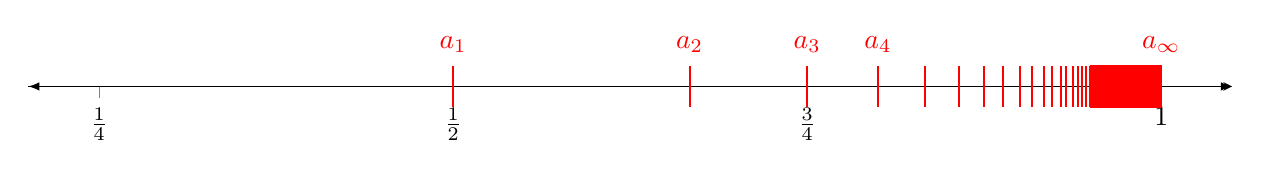
\begin{tikzpicture}
        \begin{axis}[axis y line = none, width = 2*\axisdefaultwidth, 
        height = 0.25*\axisdefaultwidth, axis lines = center, 
        xtick align = outside, xmin = 0.2, xmax = 1.05, 
        xtick = {0.25, 0.5, 0.75, 1}, xticklabels = {$\frac{1}{4}$, 
        $\frac{1}{2}$, $\frac{3}{4}$, $1$}, ymin = -0.5, ymax = 0.5, 
        clip = false]
        \draw[latex-latex](0.2, 0) --(1.05,0);
        \draw[red, thick] (0.5, -0.5) -- (0.5, 0.5);
        \draw[red, thick] (0.667, -0.5) -- (0.667, 0.5);
        \draw[red, thick] (0.75, -0.5) -- (0.75, 0.5);
        \draw[red, thick] (0.8, -0.5) -- (0.8, 0.5);
        \draw[red, thick] (0.833, -0.5) -- (0.833, 0.5);
        \draw[red, thick] (0.857, -0.5) -- (0.857, 0.5);
        \draw[red, thick] (0.875, -0.5) -- (0.875, 0.5);
        \draw[red, thick] (0.888, -0.5) -- (0.888, 0.5);
        \draw[red, thick] (0.9, -0.5) -- (0.9, 0.5);
        \draw[red, thick] (0.909, -0.5) -- (0.909, 0.5);
        \draw[red, thick] (0.917, -0.5) -- (0.917, 0.5);
        \draw[red, thick] (0.923, -0.5) -- (0.923, 0.5);
        \draw[red, thick] (0.929, -0.5) -- (0.929, 0.5);
        \draw[red, thick] (0.933, -0.5) -- (0.933, 0.5);
        \draw[red, thick] (0.9375, -0.5) -- (0.9375, 0.5);
        \draw[red, thick] (0.941, -0.5) -- (0.941, 0.5);
        \draw[red, thick] (0.944, -0.5) -- (0.944, 0.5);
        \draw[red, thick] (0.947, -0.5) -- (0.947, 0.5);
        \draw[red, thick] (0.95, -0.5) -- (0.95, 0.5);
        \filldraw[red](0.95, -0.5) rectangle (1, 0.5);
        \node[red] at (0.5, 1) {$a_1$};
        \node[red] at (0.667, 1) {$a_2$};
        \node[red] at (0.75, 1) {$a_3$};
        \node[red] at (0.8, 1) {$a_4$};
        \node[red] at (1, 1) {$a_{\infty}$};
        \end{axis}
\end{tikzpicture}
    \caption{$a_n =\frac{n}{n+1}$ on a number line}
    \label{fig:linefrac}
\end{figure}

\begin{figure}[htbp]
\centering
    \begin{tikzpicture}
        \begin{axis}[axis lines = center, xmin = -0.5, xmax = 15, 
        ymin = -0.5, ymax = 1.5, xlabel=$n$, ylabel = $a_n$]
        \addplot[blue, dashed] coordinates {(0, 1) (15, 1)};
        \addplot[mark=*, red] (1, 0.5);
        \addplot[mark=*, red] (2, 0.667);
        \addplot[mark=*, red] (3, 0.75);
        \addplot[mark=*, red] (4, 0.8);
        \addplot[mark=*, red] (5, 0.833);
        \addplot[mark=*, red] (6, 0.857);
        \addplot[mark=*, red] (7, 0.875);
        \addplot[mark=*, red] (8, 0.888);
        \addplot[mark=*, red] (9, 0.9);
        \addplot[mark=*, red] (10, 0.909);
        \addplot[mark=*, red] (11, 0.917);
        \addplot[mark=*, red] (12, 0.923);
        \addplot[mark=*, red] (13, 0.929);
        \addplot[mark=*, red] (14, 0.933);
        \addplot[mark=*, red] (15, 0.9375);
        \end{axis}
\end{tikzpicture}
    \caption{$a_n =\frac{n}{n+1}$ on an $xy$-plane}
    \label{fig:planefrac}
\end{figure}

Because $a_n$ approaches a specific number as $n \to \infty$, we call 
the series $a_n = \frac{n}{n+1}$ \textit{convergent}. We prove a 
sequence is convergent by taking the limit as $n$ approaches 
$\infty$. If the limit exists and approaches a specific number, the 
sequence is convergent. If the limit does not exist or approaches 
$\pm\infty$, the sequence is divergent. 

We can see graphically that $\lim_{n \to \infty} \frac{n}{n+1} = 1$, 
so that sequence is convergent. What about $b_n = \frac{n}{\sqrt{10 + 
n}}$? Is $b_n$ convergent or divergent? 
$$\lim_{n \to \infty} \frac{n}{\sqrt{10 + n}} = 
\lim_{n \to \infty} \frac{n/n}{\sqrt{\frac{10}{n^2}+ \frac{n}{n^2}}}$$
$$=\lim_{n \to \infty} \frac{1}{\sqrt{\frac{10}{n^2}+\frac{1}{n}}} = \infty$$

Therefore, the sequence $b_n = \frac{n}{\sqrt{10 + n}}$ is divergent. 

Here is another example of a divergent sequence: $c_n = 
\sin{\frac{n\pi}{2}}$. The graph is shown in figure \ref{fig:sineseq}. 
As you can see, the value of $c_n$ oscillates between 1, 0, and -1 
without approaching a specific number. This means that $c_n$ does 
not approach a particular number as $n \to \infty$ and the sequence is 
divergent. 

\begin{figure}[htbp]
\centering
    \begin{tikzpicture}
        \begin{axis}[axis lines = center, xmin = -0.5, xmax = 8, 
        ymin = -1.5, ymax = 1.5, xlabel=$n$, ylabel = $c_n$]
        \addplot[mark=*, red] (1, 1);
        \addplot[mark=*, red] (2, 0);
        \addplot[mark=*, red] (3, -1);
        \addplot[mark=*, red] (4, 0);
        \addplot[mark=*, red] (5, 1);
        \addplot[mark=*, red] (6, 0);
        \addplot[mark=*, red] (7, -1);
        \addplot[mark=*, red] (8, 0);
        \end{axis}
\end{tikzpicture}
    \caption{$c_n =\sin{\frac{n\pi}{2}}$ on an $xy$-plane}
    \label{fig:sineseq}
\end{figure}

\begin{Exercise}[label=seqcalc3]
Classify each sequence as convergent or divergent. If the sequence is 
convergent, find the limit as $n \to \infty$.
\begin{enumerate}
\item $a_n = \frac{3 + 5n^2}{n + n^2}$
\item $a_n = \frac{n^4}{n^3 - 2n}$
\item $a_n = 2 + (0.86)^n$
\item $a_n = \cos{\frac{n\pi}{n+1}}$
\item $a_n = \sin{n}$
\end{enumerate}
\end{Exercise}

\begin{Answer}[ref=seqcalc3]
\begin{enumerate}
\item convergent, 5
\item divergent
\item convergent, 2
\item convergent, -1
\item divergent
\end{enumerate}
\end{Answer}

\section{Evaluating limits of sequences}
Recall that a sequence can be considered a function where the domain 
is restricted to positive integers. If there is some $f(x)$ such that 
$a_n = f(n)$ when $n$ is an integer, then $\lim_{n \to \infty} a_n = 
\lim_{x \to \infty} f(x)$ (see figure \ref{fig:limit}). This means 
that all the rules that apply to the limits of functions also apply 
to the limits of sequences, including the Squeeze Theorem and 
l'Hospital's rule. 

What is $\lim_{n \to \infty} \frac{\ln{n}}{n}$? First, we will try to 
compute the limit directly:
$$\lim_{n \to \infty} \frac{\ln{n}}{n} = $$
$$\frac{\lim_{n \to \infty} \ln{n}}{\lim_{n \to \infty}n} = 
\frac{\infty}{\infty}$$

This is undefined, but fits the criteria for Ll'Hospital's rule:
$$\lim_{n \to \infty} \frac{\ln{n}}{n} = \lim_{n \to \infty} 
\frac{\frac{d}{dn}\ln{n}}{\frac{d}{dn}n}$$
$$= \lim_{n \to \infty} \frac{\frac{1}{n}}{1} = 0$$

\begin{figure}[htbp]
\centering
    \begin{tikzpicture}
        \begin{axis}[axis lines = center, xmin = -0.5, xmax = 8.5, 
        ymin = 0, ymax = 2, xlabel=$n$, ylabel = $a_n$]
        \addplot[mark=*, red] (1, 2);
        \addplot[mark=*, red] (2, 1.5);
        \addplot[mark=*, red] (3, 1.333);
        \addplot[mark=*, red] (4, 1.25);
        \addplot[mark=*, red] (5, 1.2);
        \addplot[mark=*, red] (6, 1.167);
        \addplot[mark=*, red] (7, 1.143);
        \addplot[mark=*, red] (8, 1.125);
        \draw[blue, dashed, thin] (0, 1) -- (8, 1);
        \addplot[red, domain = 0.01:8] {1+1/x};
        \end{axis}
\end{tikzpicture}
    \caption{The limit of the function is the same as the limit of the sequence}
    \label{fig:limit}
\end{figure}

Here's an example that requires the Squeeze Theorem: is the sequence 
$a_n = \frac{n!}{n^n}$ convergent or divergent? First trying to take 
the limit directly, we see that:
$$\lim_{n \to \infty} \frac{n!}{n^n} = \frac{\infty}{\infty}$$

which is undefined. Because the factorial cannot be described as a 
continuous function, we can't use l'Hospital's rule. We can examine 
this sequence graphically (see figure \ref{fig:factorial}) and 
mathematically. We examine it mathematically by writing out a few 
terms to get an idea of what happens to $a_n$ as $n$ gets large:
$$a_1 = \frac{1!}{1^1} = 1$$
$$a_2 = \frac{2!}{2^2} = \frac{1 \cdot 2}{2 \cdot 2}$$
$$a_3 = \frac{3!}{3^3} = \frac{1 \cdot 2 \cdot 3}{3 \cdot 3 \cdot 3}$$
$$\cdots$$
$$a_n = \frac{n!}{n^n} = \frac{1 \cdot 2 \cdot 3 \cdots \cdot n}{n 
\cdot n \cdot n \cdots n}$$

From examining the graph in figure \ref{fig:factorial}, we can guess 
that $\lim_{n \to \infty} a_n = 0$. Let's prove that mathematically. 
We can rewrite our expression for $a_n$ as $n$ gets large:
$$a_n = \frac{n!}{n^n} = \frac{1 \cdot 2 \cdot 3 \cdots \cdot n}{n 
\cdot n \cdot n \cdots n} = \frac{1}{n}(\frac{2 \cdot 3 \cdots n}{n 
\cdot n \cdots n})$$

The expression inside the parentheses is less than 1, therefore $0 < 
a_n < \frac{1}{n}$. Since $lim_{n \to \infty} 0 = 0$ and $\lim_{n \to 
\infty} \frac{1}{n} = 0$, by Squeeze Theorem we know that $\lim_{n 
\to \infty} \frac{n!}{n^n} = 0$. Therefore, the sequence $a_n = 
\frac{n!}{n^n}$ is convergent. 

\begin{figure}[htbp]
\centering
    \begin{tikzpicture}
        \begin{axis}[axis lines = center, xmin = -0.5, xmax = 8.5, 
        ymin = 0, ymax = 1, xlabel=$n$, ylabel = $a_n$]
        \addplot[mark=*, red] (1, 1);
        \addplot[mark=*, red] (2, 0.5);
        \addplot[mark=*, red] (3, 0.222);
        \addplot[mark=*, red] (4, 0.09375);
        \addplot[mark=*, red] (5, 0.0384);
        \addplot[mark=*, red] (6, 0.01543);
        \addplot[mark=*, red] (7, 0.00612);
        \addplot[mark=*, red] (8, 0.0024);
        \end{axis}
\end{tikzpicture}
    \caption{$a_n = \frac{n!}{n^n}$}
    \label{fig:factorial}
\end{figure}

[[FIX ME intro]]
If $\lim_{n \to \infty} a_n = L$ and the function $f$ is continuous 
at $L$, then $\lim_{n \to \infty} f(a_n) = f(L)$. For example, what 
is $\lim_{n \to \infty} \sin{\frac{\pi}{n}}$? Well, we know that 
$\lim_{n \to \infty} \frac{\pi}{n} = 0$ and that the sine function is 
continuous at 0. Therefore, $\lim_{n \to \infty} \sin{\frac{\pi}{n}} 
= \sin{\lim_{n \to \infty} \frac{\pi}{n}} = \sin{0} = 0$. 

\section{Monotonic and Bounded sequences}
Just like functions, sequences can be increasing or decreasing. A 
sequence is increasing if $a_n < a_{n+1}$ for $n \geq 1$. Similarly, 
a sequence is decreasing if $a_n > a_{n+1}$ for $n \geq 1$. If a 
sequence is strictly increasing or decreasing, it is called 
\textit{monotonic}. 

The sequence $a_n = \frac{1}{n + 6}$ is decreasing. We prove this 
formally by comparing $a_n$ to $a_{n+1}$:
$$\frac{1}{n + 6} > \frac{1}{(n + 1) + 6} = \frac{1}{n + 7}$$

Is the sequence $a_n = \frac{n}{n^2 + 1}$ increasing or decreasing? 
First, we find an expression for $a_{n+1}$:
$$a_{n + 1} = \frac{n + 1}{(n + 1)^2 + 1} = \frac{n + 1}{n^2 + 2n + 2}$$

Since the degree of $n$ is greater in the denominator, we have a guess 
that the sequence is decreasing. To prove this, we check if $a_n > 
a_{n+1}$ is true:
$$\frac{n}{n^2 + 1} > \frac{n + 1}{n^2 + 2n + 2}$$

We can cross-multiply, because $n > 0$ and the denominators are 
positive:
$$(n)(n^2 + 2n + 2) > (n+1)(n^2 + 1)$$
$$n^3 + 2n^2 + 2n > n^3 + n^2 + n + 1$$

Subtracting $(n^3 + n^2 + n)$ from both sides we see that:
$$n^2 + n > 1$$

Which is true for all $n \geq1$. Therefore, $a_n > a_{n+1}$ for all 
$n \geq 1$ and the sequence is decreasing. 

A sequence is \textit{bounded above} if there is some number $M$ such 
that $a_n \leq M$ for all $n \geq 1$. And a sequence is 
\textit{bounded below} if there is some other number $m$ such that 
$a_n \geq m$ for all $n \geq 1$. If a sequence is bounded above and 
below, then it is a \textit{bounded sequence}. 

If a sequence is both \textit{monotonic} and \textit{bounded}, then it 
must be convergent. 

Example: is the sequence given by $a_n = 4$ and $a_{n+1} = \frac{1}{2}
(a_n + 7)$ bounded above, below, both, or neither?

We start by calculating the first several terms:
\begin{center}
	\begin{tabular}{|c|c|c|}\hline
	Term & Work & Value\\
	\hline
	$a_1$ & $a_1 = 4$ & 4\\
	\hline
	$a_2$ & $=\frac{1}{2}(4 + 7)$ & 5.5\\
	\hline
	$a_3$ & $=\frac{1}{2}(5.5+7)$ & 6.25\\
	\hline
	$a_4$ & $=\frac{1}{2}(6.25+7)$ & 6.625\\
	\hline
	$a_5$ & $=\frac{1}{2}(6.625+7)$ & 6.8125\\
	\hline
	$a_6$ & $=\frac{1}{2}(6.8125+7)$ & 6.90625\\
	\hline
	$a_7$ & $=\frac{1}{2}(6.90625+7)$ & 6.953125\\
	\hline
	$a_8$ & $=\frac{1}{2}(6.953125+7)$ & 6.9765625\\
	\hline	
	\end{tabular}
\end{center}

The sequence is increasing, so it is bounded below by the initial 
term, $a_1 = 4$, and we can state that $a_n \geq 4$. Examining the 
computed terms, we see that $a_n \to 7$ as $n$ grows larger. We can 
guess that this sequence is bounded above, with $a_n \leq 7$. We can 
prove this by induction. Suppose that there is some $k$ such that 
$a_k < 7$ (which is true for $a_1$, etc.). Then
$$a_k < 7$$
$$a_k + 7 < 14$$
$$\frac{1}{2}(a_k + 7) < \frac{1}{2}(14)$$
$$a_{k + 1} < 7$$\\
Therefore, $a_n < 7$ for all $n$ and the sequence is bounded above. 
Because the sequence is monotonic and bounded, we know the sequence 
is convergent and, therefore, that the limit of $a_n$ as $n \to 
\infty$ exists. 

\section{Applications of Sequences}
\subsection{Compound Interest}
When you put money in a bank account or invest it, your money may 
accumulate \textit{compound interest}. Compound interest is interest 
paid on the principal (the amount you originally invested) and 
previously accumulated interest. For example, suppose you put \$100 
in a savings account that earns 3.25\% annually. After one year, the 
bank will pay $(\$100)\cdot (0.0325) = \$3.25$ into your savings 
account. Now you have \$103.25. The \textit{next} year, your bank will 
pay you 3.25\% interest on the entire amount in your bank account 
(the \$100 principal plus the \$3.25 in earned interest). This comes 
to $\$103.25 \cdot 0.0325 = \$3.36$ and your new account total will be 
\$106.61. This continues year over year and can build up quite a bit 
of money. How can we model compound interest as a sequence? Let's 
write out how we calculate the first few years of interest 
accumulation:
$$a_0 = 100\text{ (this represents our principal investment)}$$
$$a_1 = a_0 + a_0(0.0325)\text{ (the total value of the bank account 
will be the previous year's value plus the interest)}$$\\
We can combine terms to see that:
$$a_1 = a_0{1.10325}$$\\
Similarly, 
$$a_2 = a_1(1.0325) = [a_0(1.0325)](1.0325) = a_0(1.0325)^2$$
$$a_3 = a_2(1.0325) = [a_0(1.0325)^2](1.0325) = a_0(1.0325)^3$$\\
Do you see the pattern? For an initial investment of \$100 at an 
annual rate of 3.25\% compounded annually, the value of the bank 
account at the end of the $n^{th}$ year is given by:
$$a_n = 100(1.0325)^{n}$$\\
The general form of this formula with an initial investment of $P$ 
and annual interest rate $r$ is:
$$a_n = P(1+r)^{n}$$

\begin{Exercise}[label=seqcalc5]
You invest \$1500 at 5\%, compounded annually. Write an explicit 
formula that describes the value of your investment every year. 
What will your investment be worth after 10 years? Is the sequence 
convergent or divergent? Explain. 
\end{Exercise}

\begin{Answer}[ref=seqcalc5]
Out principal is $P = 1500$ and the interest rate is $r = 0.06$. 
After $n$ years, your investment will be worth $a_n = 1500(1.06)^{n}$. 
For $n = 10$, your investment will be valued at $a_{10} = \$1500
(1.06)^{10} = \$2686.27$ (that's over \$1000 in interest!). To 
determine if the sequence is convergent or divergent, we examine the 
limit as $n \to \infty$:
$$\lim_{n \to \infty} 1500(1.06)^n = 1500\cdot \lim_{n \to \infty}
(1.06)^n = 1500 \cdot \infty = \infty$$\\
The sequence is divergent. 
\end{Answer}